\section{Example}

\subsection{Random Bits}

\begin{frame}
    \frametitle{Outline}
    \tableofcontents[currentsection, currentsubsection]
\end{frame}

\begin{frame}
    \frametitle{What is Mathematical Modeling?}
    \begin{figure}
        \centering
        \caption{
        \href{http://www.youtube.com/watch?v=Jzl39jqZjsw&feature=share&list=UUEWRMyobsgQG-PaC9ldME4A}{
        Trillion Dollar} 
        \href{http://www.youtube.com/watch?v=G17rx7H3DtI&feature=BFa&list=UUEWRMyobsgQG-PaC9ldME4A}{Bet}
        }
        \href{http://www.youtube.com/watch?v=dsrOXJwGwtk}{
        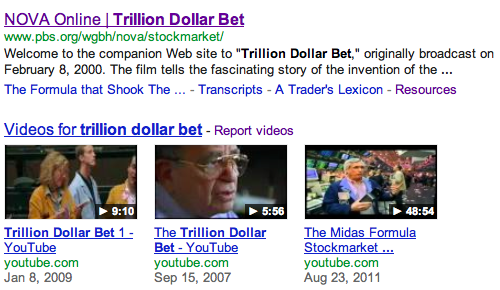
\includegraphics[width=\textwidth]{TrillionDollarBet.png}
        }
        \label{fig:LTCM}
    \end{figure}
\end{frame}

\begin{frame}
    \frametitle{What is Mathematical Modeling?}
    \begin{figure}
        \centering
        \caption{{LAPD Fighting Crime with Math}}
        \href{http://www.youtube.com/watch?v=HZ7fLuO7zb4}{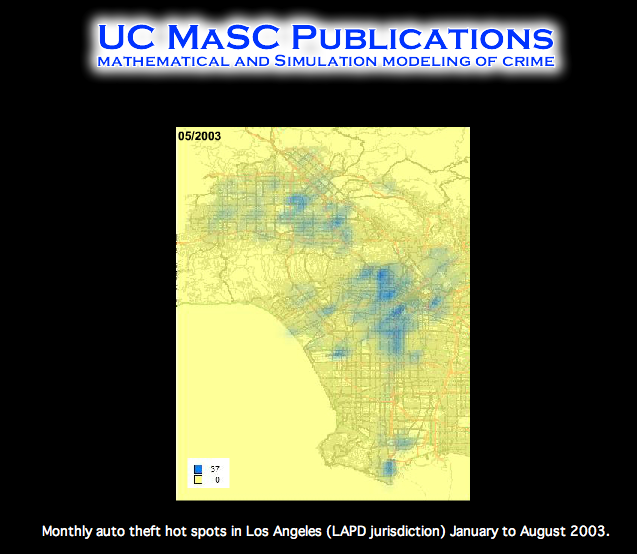
\includegraphics[width=0.6\textwidth]{LAPDUCLA.png}}
        \label{fig:LAPDUCLA}
    \end{figure}
\end{frame}

\begin{frame}[fragile]
    \frametitle{What is Mathematical Modeling?}
        \begin{figure}
            \centering
            \caption{Crime rates and religious beliefs}
            \href{http://www.economist.com/blogs/graphicdetail/2012/09/daily-chart/}{
            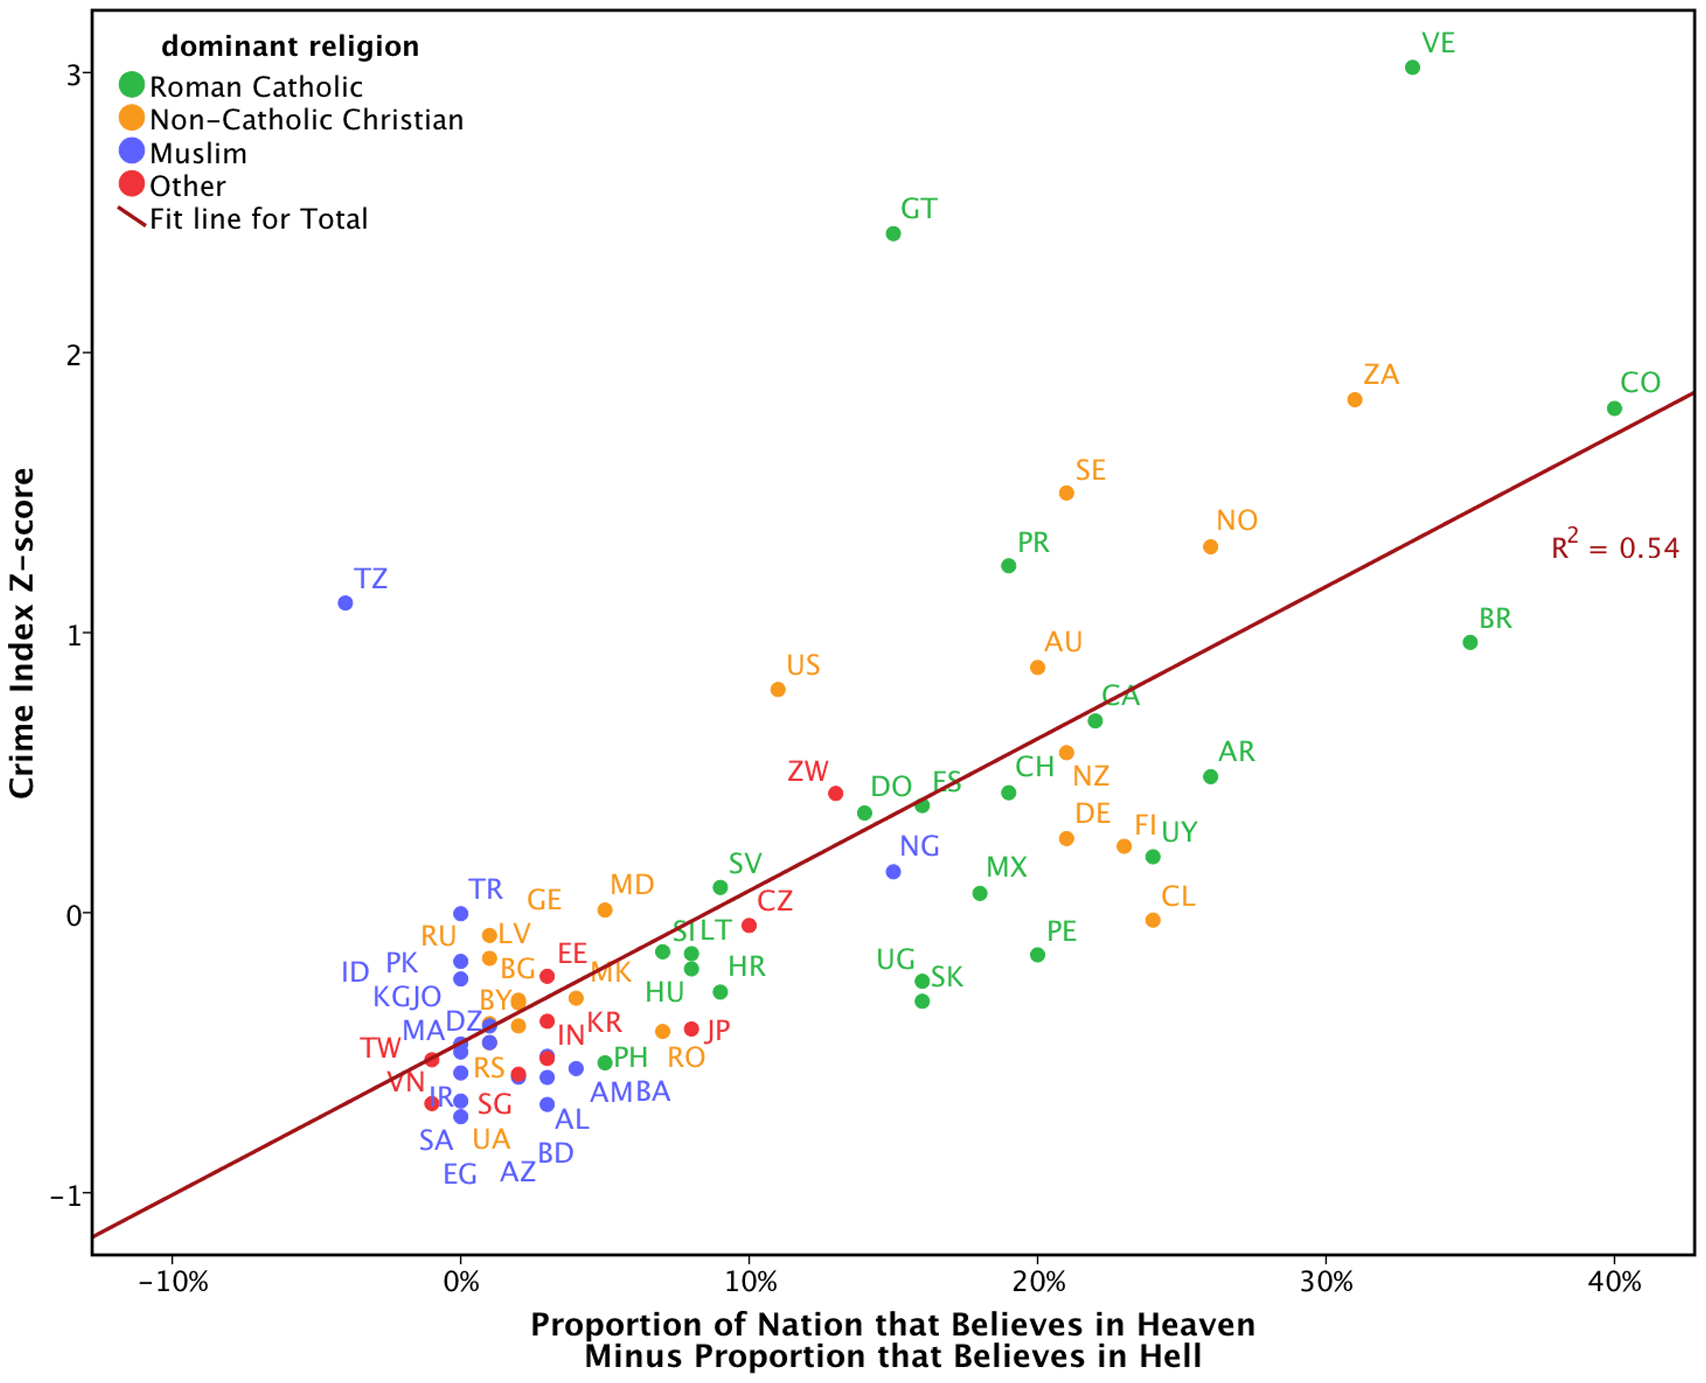
\includegraphics[width=0.7\textwidth]{images/hellvsheaven.png}}
    \end{figure}
\end{frame}

\begin{frame}[fragile]
    \frametitle{More Project Ideas}
    \begin{center}
    \href{http://www.stat.berkeley.edu/users/statlabs/}{http://www.stat.berkeley.edu/}
    \end{center}
    \vskip0.25in
    \begin{center}
        \href{http://www.math.msu.edu/Academic%5FPrograms/graduate/msim//ProjectPage.aspx}{http://www.math.msu.edu/}
    \end{center}
    \vskip0.25in
    \begin{center}
        \href{http://www.mathgoespop.com/2011/09/moneyball.html}{http://www.mathgoespop.com/}
    \end{center}
    \vskip0.25in
    \begin{center}
        \href{http://www.math.hmc.edu/clinic/projects/years/}{http://www.math.hmc.edu/clinic/}
    \end{center}
\end{frame}

\subsection{Insurance Redlining}

\begin{frame}
    \frametitle{Outline}
    \tableofcontents[currentsection, currentsubsection]
\end{frame}

\newtheorem{DEFinsredlining}{Insurance Redlining}
\newtheorem{DEFfairplan}{FAIR}
\begin{frame}
    \frametitle{ Insurance Redlining}
    \begin{DEFinsredlining}
        \textcolor{red}{Insurance redlining} refers to the practice of refusing
        to issue insurance to certain types of people or within some 
        geographic area. 
    \end{DEFinsredlining}
\vskip.5in
    \begin{DEFfairplan}
        The \textcolor{red}{FAIR} plan was offered by the city of Chicago as a 
        default policy to homeowner who had been rejected by the voluntary
        market. 
    \end{DEFfairplan}
\end{frame}

\begin{frame}
    \frametitle{ Insurance Redlining}
    \begin{figure}
        \centering
        \caption{Insurance Redlining}
        \href{http://en.wikipedia.org/wiki/Redlining}{
        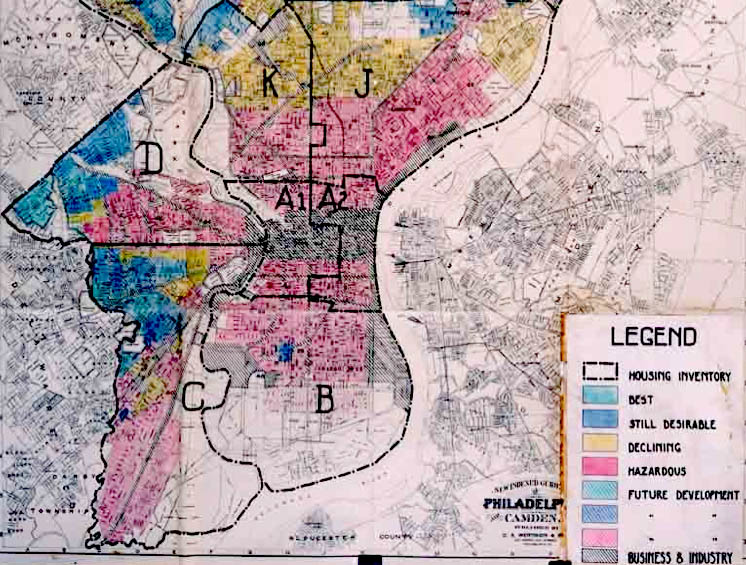
\includegraphics[width=0.8\textwidth]{redliningPhilly.jpg}
        }
                \label{fig:redlining}
    \end{figure}
\end{frame}



\newtheorem{DEFsponsorUSCCR}{Sponsor}
\newtheorem{DEFdataFAIR}{Data}
\begin{frame}
    \frametitle{ Insurance Redlining}
    \begin{DEFsponsorUSCCR} 
        The \href{http://www.usccr.gov/about/}{\textcolor{red}{U.S.~Commission
        on Civil Rights}} examined 
        charges by several Chicago community organizations that insurance 
        companies were redlining their neighborhoods. 
    \end{DEFsponsorUSCCR}
    \vskip.5in
    \begin{DEFdataFAIR}
        The \textcolor{red}{number of FAIR plan policies} written and renewed in Chicago
        by zip code for the number of months of December 1977 through May
        1978.
    \end{DEFdataFAIR}
\end{frame}

\begin{frame}
    \frametitle{ Insurance Redlining}
    Variables to consider:
    \begin{description}
        \item[\texttt{race}] Racial composition in percentage of minority,
        \item[\texttt{fire}] Fire per 100 housing units,
        \item[\texttt{theft}] Theft per 1000 population,
        \item[\texttt{age}] percent of housing unit built before 1939,
        \item[\texttt{involact}] New FAIR plan policies and renewal per 100 housing units,
        \item[\texttt{income}] Median family income in thousands of dollars,
        \item[\texttt{side}] North or South side of Chicago.
    \end{description}
\end{frame}

\newtheorem{DEFecofallacy}{Ecological Fallacy}
\begin{frame}
    \frametitle{Insurance Redlining: Ecological Fallacy}
    \begin{DEFecofallacy}
       When data are collected at the group level, we may observe 
       a correlation between two variables.  The \textcolor{red}{ecological
       fallacy} is concluding that the same correlation holds at the
       individual level. 
    \end{DEFecofallacy}
\end{frame}

\begin{frame}
    \frametitle{Insurance Redlining: Ecological Fallacy}
    \begin{figure}
        \centering
        \caption{1998 annual per capita income and proportion U.S.~born for 50
        states plus D.C.}
        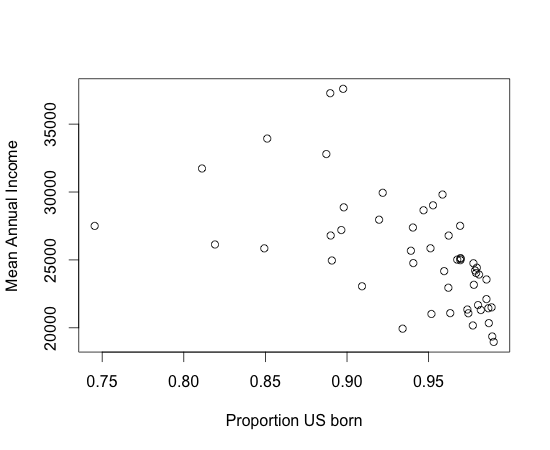
\includegraphics[width=0.75\textwidth]{images/FigureFarawayFigure11dot1.png}
    \end{figure}
\end{frame}

\begin{frame}
    \frametitle{Insurance Redlining: Ecological Fallacy}
    \begin{figure}
        \centering
        \caption{1998 annual per capita income and proportion U.S.~born for 50
        states plus D.C.}
        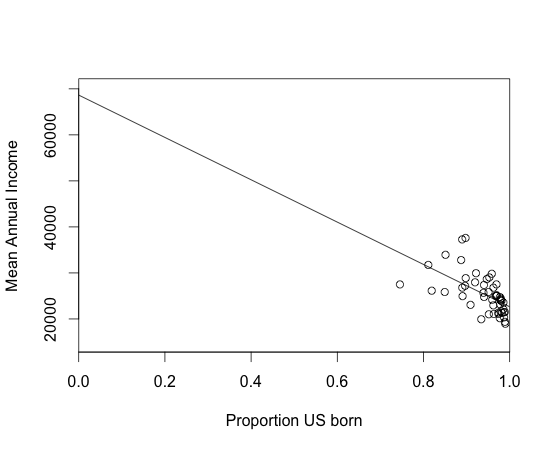
\includegraphics[width=0.75\textwidth]{images/FigureFarawayFigure11dot1b.png}
    \end{figure}
\end{frame}

\begin{frame}[fragile]
    \frametitle{ Insurance Redlining}
    \begin{verse}
For the ecological fallacy example, 
the assumption would be that the incomes of 
the native born do not depend on the proportion of native 
born within the state (and similarly for naturalized citizens).
    \end{verse}
    \vskip0.5in
    \begin{verse}
        For the insurance redlining example, we only have aggregate data.  
        We must inform the sponsor that unless more detailed data becomes
        available, the results for the aggregated data may not hold true 
        at the individual level. 
    \end{verse}
\end{frame}

\begin{frame}[fragile]
    \frametitle{Work Statement: Introduction}
    The work statement should contain a short description 
    of your sponsor.  
    \vskip0.2in
    For the insurance redlining example, 
    \emph{U.S.~Commision on Civil Rights} would be the sponsor.
    \vskip0.2in
    \href{http://en.wikipedia.org/wiki/Boilerplate_%28text%29}{\emph{Boilerplating}} from the sponsor's webpage is often acceptable. 
    \vskip0.5in
    \begin{center}
        \href{http://www.usccr.gov/about/}{http://www.usccr.gov}
    \end{center}
\end{frame}


\begin{frame}   
    \frametitle{Work Statement: Problem Statement}
    \begin{verse}
        Can the insurance companies claim that the discrepancy is due to 
        greater risks in some zip codes?
    \end{verse}
    \vskip0.5in
    \begin{verse}
        The insurance companies could claim that they were denying insurance 
        in neighborhoods where they had sustained large fire-related losses
        and any discriminatory effect was a by-product of legitimate business
        practice.  
    \end{verse}
\end{frame}


\subsection{Sherlock Holmes and the Bicycle Tracks}

\begin{frame}
    \frametitle{Outline}
    \tableofcontents[currentsection, currentsubsection]
\end{frame}

\begin{frame}
    \frametitle{Sherlock Holmes and the Bicycle Tracks: Problem Statement}
    \begin{figure}
        \caption{Which one is the front wheel?}
        \begin{center}
            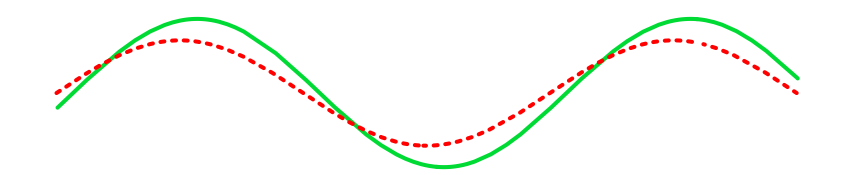
\includegraphics[width=\textwidth]{images/sholmesbike.png}
        \end{center}
        \label{fig:sholmesbike}
    \end{figure}
\end{frame}


\begin{frame}
    \frametitle{Sherlock Holmes and the Bicycle Tracks}
    \begin{verse}
        ``This track, as you perceive, was made by a rider who was going from
        the direction of the school.''
    \end{verse}
    \begin{verse}
        ``Or Toward it?''
    \end{verse}
    \begin{verse}
        ``No, no, my dear Watson.  The more deeply sunk impression is, of
        course, the hind wheel, upon which the weight rests.  You perceive
        several places where it has passed across and obliterated the more
        shallow mark of the front one.  It was undoubtedly heading away from
        the school.''
    \end{verse}
    \hfill -- \textit{The Adventure of the Priory School} by Arthur Conan Doyle
\end{frame}

\begin{frame}
    \frametitle{Sherlock Holmes and the Bicycle Tracks}
    \begin{align*}
        &f_x(t) = r_x(t) +
        \dfrac{L}{\sqrt{1+(r_y^\prime(t)/r_x^\prime(t))^2}}\\
        &f_y(t) = r_y(t) + \dfrac{L r_y^\prime(t)/r_x^\prime(t)}{
        \sqrt{1+ (r_y^\prime(t)/r_x^\prime(t))^2}}
    \end{align*}
\end{frame}

\subsection{Fair Play}
\begin{frame}
    \frametitle{Outline}
    \tableofcontents[currentsection, currentsubsection]
\end{frame}

\begin{frame}
    \frametitle{Is a Sport Game Fair?: Problem Statement}
    \begin{figure}
        \caption{
            \href{http://www.youtube.com/watch?v=WNlCBy07z08}{
            How can we decide if a game with two competitors is fair?}
            }
            \centering
            \href{avmedia/nprnewssports.mp3}{
            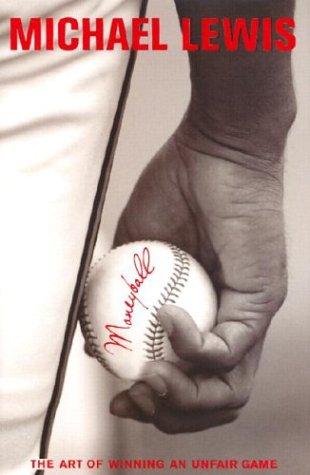
\includegraphics[width=0.4\textwidth]{Moneyballs.jpg}
            }
    \end{figure}
\end{frame}

\begin{frame}
    \frametitle{Is a Tennis Match Fair?}
    One simple answer is: 
    \vskip0.2in
    \begin{verse}
        If the roles of the competitors are reversed,
        their probability of winning does not change.
    \end{verse}
    \vskip0.2in
    Isn't that always true?  No.  For example, going first may give a player
    an advantage of disadvantage.
\end{frame}

\begin{frame}
    \frametitle{Is a Tennis Match Fair?: Problem Statement}
    \begin{figure}
        \caption{How can we decide if a game with two competitors is fair?}
        \begin{center}
            \href{http://www.youtube.com/watch?v=ekQ_Ja02gTY}{
            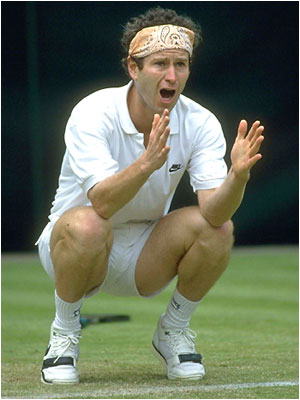
\includegraphics[width=0.4\textwidth]{images/jmcenroe.jpg}}
        \end{center}
        \label{fig:FairGame}
    \end{figure}
\end{frame}

\begin{frame}
    \frametitle{Is Tennis Fair?}
    Review of our work done last time. 
    \begin{itemize}
        \item What is tennis (for our mathematical modeling purpose)? 
        \item What was assumed to be ignored? 
        \item How was the server's advantage modeled? 
        \item What did we do to simplify our model? 
        \item Is there a ``generalized'' rule that models the tennis set
            winning determination? 
        \item Who could be your sponsor/client? (Try \href{http://www.usta.com/About-USTA/?intloc=headernav}{USTA})
    \end{itemize}
\end{frame}
